\documentclass[paper=a5,DIV=15,headinclude,twoside=semi,openany,titlepage=firstiscover]{scrbook}
\usepackage[utf8]{inputenc}
\usepackage[T1]{fontenc}
\usepackage[swedish]{babel}
\usepackage{lipsum}
\title{En liten guide för att skriva fallrapport}
\author{T. Tolvansson}
\date{October 2020}
\usepackage{calc}
\usepackage[dvipsnames]{xcolor}
\usepackage{tikz}
\usetikzlibrary{shapes}
\usetikzlibrary{calc}
\usepackage{anyfontsize}
%\usepackage{sectsty}
\usepackage[lf]{linguisticspro}
\usepackage{Rosario}
\usepackage{paralist}
\usepackage{array}
\usepackage{xhfill}
\lowertitleback{%
test text

}
\newcommand{\siffergrey}{black!50!white}

%\newcommand{\sifferlinje}[1]{%
%	\noindent\textcolor{black!50!white}{{\huge  \textcolor{\siffergrey}{#1}}\xrfill[.5ex]{2pt}[\siffergrey]}}
%}

\newcommand{\sifferlinje}[1]{%
	\noindent{\large\textcolor{black}{#1}}\xrfill[0ex]{1pt}
}

\begin{document}
\frontmatter
\begin{titlepage}
\begin{tikzpicture}[remember picture,overlay]
%\fill[BlueViolet] (current page.south west) rectangle (current page.north east);
%%% NEDRE VÄNSTER
\begin{scope}
\foreach \i in {2.5,...,15.5}
{\node[rounded corners,black!30,draw,regular polygon,regular polygon sides=6, minimum size=\i cm,ultra thick] at ($(current page.west)+(2.5,-5)$) {} ;}
\end{scope}

%%% ÅR
%\node[rounded corners,text=black!60,regular polygon,regular polygon sides=6, minimum size=2.5 cm,inner sep=0,ultra thick] at ($(current page.west)+(2.5,-5)$) {\LARGE \bfseries 2020};

\node (myfirstpic) at ($(current page.west)+(2.5,-5)$) {
\includegraphics[scale=0.12]{coverfallrisksymbol}};

%%% Uppe vänster
\foreach \i in {0.5,...,18}
{\node[rounded corners,black!30,draw,regular polygon,regular polygon sides=6, minimum size=\i cm,ultra thick] at ($(current page.north west)+(2.5,0)$) {} ;}

%%% Höger uppe
\foreach \i in {0.5,...,15}
{\node[rounded corners,black!10,draw,regular polygon,regular polygon sides=6, minimum size=\i cm,ultra thick] at ($(current page.north east)+(0,-9.5)$) {} ;}

%%% nere höger centrum
%\foreach \i in {5}
%{\node[rounded corners,draw=black!70,regular polygon,regular polygon sides=6, minimum size=\i cm,ultra thick] at ($(current page.south east)+(-0.2,-0.45)$) {} ;}

%%% nere höger hexagon
\foreach \i in {12,...,0.5}
{\node[black!20,rounded corners,draw,regular polygon,regular polygon sides=6, minimum size=\i cm,ultra thick] at ($(current page.south east)+(-0.2,-0.45)$) {} ;}

%%% TEXTER


%%% 
%\node[left,black,minimum width=0.625*\paperwidth,minimum height=2cm, rounded corners] at ($(current page.north east)+(-2,-11)$){{\huge \textit{Subtitle of the Report}}};

\node[black,minimum width=0.625*\paperwidth,minimum height=2cm, rounded corners] at ($(current page.north east)+(-4,-7)$){{\LARGE \textit{En liten guide till}}};

\node[black,minimum width=0.625*\paperwidth,minimum height=3cm, rounded corners] at ($(current page.north east)+(-5,-8.25)$){{\fontsize{25}{30} \selectfont \bfseries att skriva fallrapporter}};

\end{tikzpicture}
\end{titlepage}

\mainmatter
\pagestyle{empty}

\section*{När ska en fallrapport skrivas?}
\textit{Varje gång en brukare oavsiktligen hamnar på golvet}. Det kan vara att tappa balansen och trilla, men också att glida ur sängen eller att benen viker sig när man reser sig från toaletten. Om brukaren hamnar på golvet, och det inte var avsiktligt, ska en fallrapport skrivas.

\section*{Vad ska jag göra efter en fallhändelse?}
Sjuksköterska ska kontaktas, och en fallhändelsen ska dokumenteras i Procapita.

\section*{Varför skriver vi fallrapporter?}
Genom att dokumentera fallhändelser kan vi försöka se mönster och systematiskt hitta orsaker och åtgärder med syfte att förhindra fler fall. 

\clearpage

%\begin{enumerate}
%    \item Klicka på ”Komponenter” i navigeringsfliken.\\ 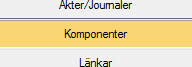
\includegraphics{fall1}
%    \item Dubbelklicka på ”Avvikelser”\\ 
\includegraphics{fall2}
%    \item Fyll i personnummer och klika på ikonen ”kikare”
%    \item Klicka på ikonen ”ny”
%    5\item Kontrollera att organisationen stämmer
%    \item Välj avvikelse ”HSL - Fallhändelse” i rull-listan.
%    \item Välj mottagare ”Vevrehemmet Äbo - HSL” eller ”Vevrehemmet Dembo - HSL”
%    \item Fyll i all information nedan. ”Pågick till” och ”Medanmälare” är frivilligt. Obs! Händelsedatum och -tid anger när fallet inträffade, inte när det upptäcktes.
%    \item Klicka på fliken ”Ytterligare uppgifter”
%    10\item Fyll i all information nedan förutom ”Allvarlighetsgrad”.
%    \item Klicka på ikonen ”Spara”.
%    \item Klicka på fliken ”Dokumentation”
%    \item Öppna ”Avvikelse HSL” och dokumentera under ”Beskrivning av händelseförloppet.” (Läs mer om detta på nästa sida.)
%    \item Klicka på ikonen ”Spara”.
%    \item Signera när rutan för signering kommer upp på skärmen.
%\end{enumerate}

\section*{Steg för steg i Procapita}
%\sifferlinje{1}
%\indent \hrulefill
\noindent\hrulefill
%%% 1.
\vfill
\noindent
\begin{minipage}[t]{0.06\textwidth}
\phantom{1}1.
\end{minipage}%
\begin{minipage}[t]{.49\textwidth}
Klicka på ``\textbf{Komponenter}'' i\\ navigeringsfliken.
\end{minipage}% This must go next to `\end{minipage}`
\begin{minipage}[t]{.45\textwidth}
\hfill\raisebox{-\height+0.7\baselineskip}{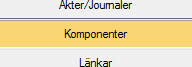
\includegraphics[scale=1]{fall1}}
\end{minipage}
\vfill

\noindent\hrulefill

%%% 2
\vfill
\noindent
\begin{minipage}[t]{0.06\textwidth}
\phantom{1}2.
\end{minipage}%
\begin{minipage}[t]{.49\textwidth}
	Dubbelklicka på ``\textbf{Avvikelser}''.
\end{minipage}%
\begin{minipage}[t]{.45\textwidth}
	\hfill\raisebox{-\height+0.7\baselineskip}{
\includegraphics[scale=1]{fall2}}
\end{minipage}
\vfill

\noindent\hrulefill

%%% 3
\vfill
\noindent
\begin{minipage}[t]{0.06\textwidth}
	\phantom{1}3.
\end{minipage}%
\begin{minipage}[t]{.44\textwidth}
	Fyll i personnummer och\\ klicka på ikonen ``\textbf{kikare}''.
\end{minipage}% This must go next to `\end{minipage}`
\begin{minipage}[t]{.5\textwidth}
	\hfill\raisebox{-\height+0.7\baselineskip}{
\includegraphics[scale=1]{fall3}}
\end{minipage}
\vfill

\noindent\hrulefill

%%% 4
\vfill
\noindent
\begin{minipage}[t]{0.06\textwidth}
	\phantom{1}4.
\end{minipage}%
\begin{minipage}[t]{.44\textwidth}
	Klicka på ikonen ``\textbf{ny}''\\(ett vitt ark uppe till vänster).
\end{minipage}% This must go next to `\end{minipage}`
\begin{minipage}[t]{.5\textwidth}
	\hfill\raisebox{-\height+0.7\baselineskip}{
\includegraphics[scale=1]{fall4}}
\end{minipage}
\vfill

\noindent\hrulefill

%%% 5
\vfill
\noindent
\begin{minipage}[t]{0.06\textwidth}
	\phantom{1}5.
\end{minipage}%
\begin{minipage}[t]{.44\textwidth}
	Kontrollera att \textbf{organisationen} stämmer.
\end{minipage}% This must go next to `\end{minipage}`
\begin{minipage}[t]{.5\textwidth}
	\hfill\raisebox{-\height+0.7\baselineskip}{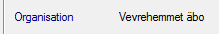
\includegraphics[scale=0.9]{fall5}}
\end{minipage}
\vfill

\noindent\hrulefill

%%% 6
\vfill
\noindent
\begin{minipage}[t]{0.06\textwidth}
	\phantom{1}6.
\end{minipage}%
\begin{minipage}[t]{.54\textwidth}
	Välj \textbf{avvikelse} ”HSL - Fallhändelse”\\
	i rull-listan.
\end{minipage}% This must go next to `\end{minipage}`
\begin{minipage}[t]{.4\textwidth}
	\hfill\raisebox{-\height+0.7\baselineskip}{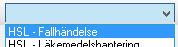
\includegraphics[scale=1]{fall6a}}
\end{minipage}
\vfill

\noindent\hrulefill

%%% 7
\vfill
\noindent
\begin{minipage}[t]{0.06\textwidth}
	\phantom{1}7.
\end{minipage}%
\begin{minipage}[t]{.54\textwidth}
	Välj \textbf{mottagare}:\\ 
	”Vevrehemmet Dembo - HSL” eller\\”Vevrehemmet Äbo - HSL”
\end{minipage}% This must go next to `\end{minipage}`
\begin{minipage}[t]{.4\textwidth}
	\hfill\raisebox{-\height+0.7\baselineskip}{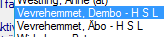
\includegraphics[scale=1.05]{fall7a}}
\end{minipage}
\vfill

\noindent\hrulefill
\newpage
\noindent\hrulefill

%%% 8
\vfill
\noindent
\begin{minipage}[t]{0.06\textwidth}
	\phantom{1}8.
\end{minipage}%
\begin{minipage}[t]{.94\textwidth}
	\textbf{Fyll i} all information på denna sida. ”Pågick till” och ”Medanmälare” är frivilligt. \textit{OBS! ``Har hemvård'' ska fyllas i ``Ja''}
\end{minipage}% This must go next to `\end{minipage}`
%\begin{minipage}[t]{.4\textwidth}
%	\hfill\raisebox{-\height+0.7\baselineskip}{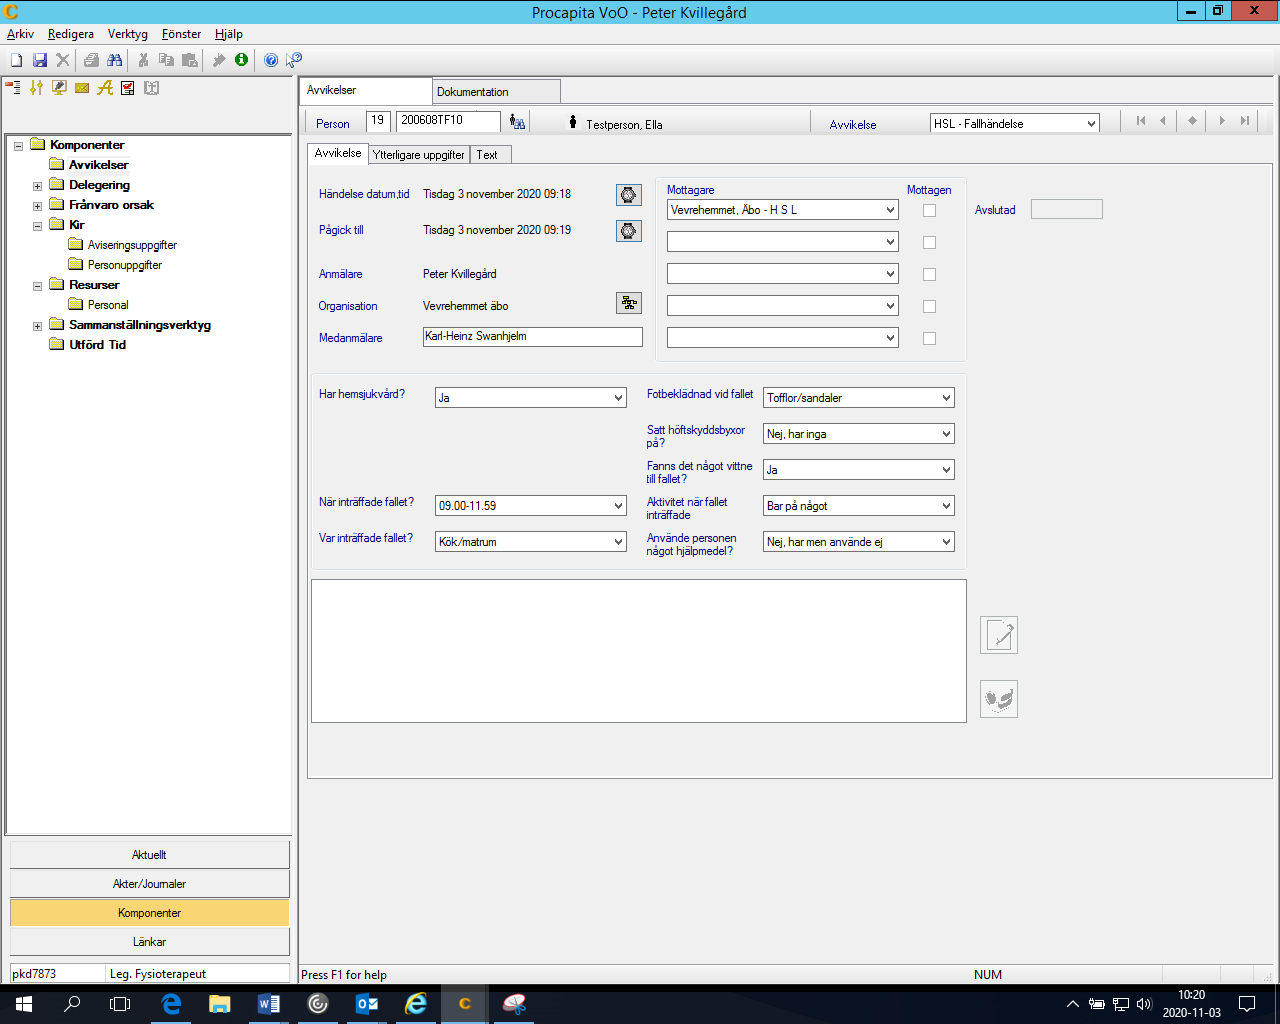
\includegraphics[scale=1.1]{fall8}}
%\end{minipage}
\vfill

\noindent\hrulefill

%%% 9
\vfill
\noindent
\begin{minipage}[t]{0.06\textwidth}
	\phantom{1}9.
\end{minipage}%
\begin{minipage}[t]{.54\textwidth}
	Klicka på fliken\\”\textbf{Ytterligare uppgifter}”
\end{minipage}% This must go next to `\end{minipage}`
\begin{minipage}[t]{.4\textwidth}
	\hfill\raisebox{-\height+0.7\baselineskip}{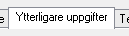
\includegraphics[scale=1]{fall9a}}
\end{minipage}
\vfill

\noindent\hrulefill

%%% 10
\vfill
\noindent
\begin{minipage}[t]{0.06\textwidth}
	10.
\end{minipage}%
\begin{minipage}[t]{.94\textwidth}
	\textbf{Fyll i} all information för ``Ytterligare uppgifter'' förutom\\ ”Allvarlighetsgrad”. \textit{OBS! Fyll inte i ``Allvarlighetsgrad''}.
\end{minipage}% This must go next to `\end{minipage}`
%\begin{minipage}[t]{.4\textwidth}
%	\hfill\raisebox{-\height+0.7\baselineskip}{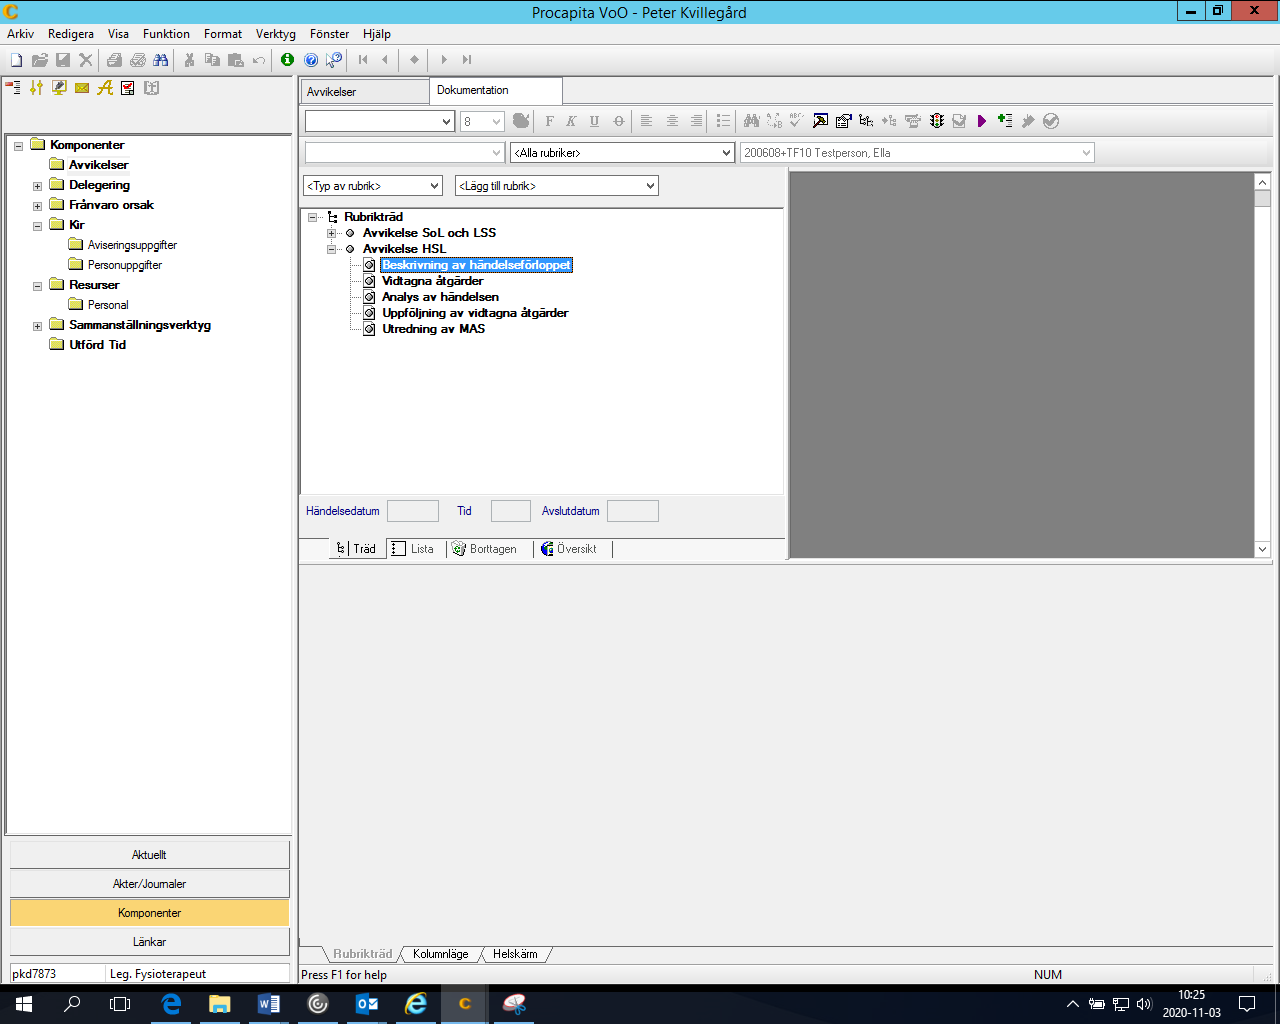
\includegraphics[scale=1]{fall10}}
%\end{minipage}
\vfill

\noindent\hrulefill

%%% 11
\vfill
\noindent
\begin{minipage}[t]{0.06\textwidth}
	11.
\end{minipage}%
\begin{minipage}[t]{.44\textwidth}
	Klicka på ikonen ”\textbf{Spara}”.
\end{minipage}% This must go next to `\end{minipage}`
\begin{minipage}[t]{.5\textwidth}
	\hfill\raisebox{-\height+0.7\baselineskip}{
\includegraphics[scale=1]{fall11a}}
\end{minipage}
\vfill

\noindent\hrulefill

%%% 12
\vfill
\noindent
\begin{minipage}[t]{0.06\textwidth}
	12.
\end{minipage}%
\begin{minipage}[t]{.44\textwidth}
	Klicka på fliken ”\textbf{Dokumentation}”
\end{minipage}% This must go next to `\end{minipage}`
\begin{minipage}[t]{.5\textwidth}
	\hfill\raisebox{-\height+0.7\baselineskip}{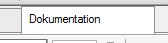
\includegraphics[scale=1]{fall12}}
\end{minipage}
\vfill

\noindent\hrulefill

%%% 13
\vfill
\noindent
\begin{minipage}[t]{0.06\textwidth}
	13.
\end{minipage}%
\begin{minipage}[t]{.45\textwidth}
	Öppna ”\textbf{Avvikelse HSL}” och dokumentera under ”\textbf{Beskrivning av händelseförloppet}”. (Läs mer om detta på nästa sida.)
\end{minipage}% This must go next to `\end{minipage}`
\begin{minipage}[t]{.49\textwidth}
	\hfill\raisebox{-\height+0.7\baselineskip}{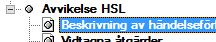
\includegraphics[scale=1]{fall13}}
\end{minipage}
\vfill

\noindent\hrulefill

%%% 14
\vfill
\noindent
\begin{minipage}[t]{0.06\textwidth}
	14.
\end{minipage}%
\begin{minipage}[t]{.44\textwidth}
	Klicka på ikonen ”\textbf{Spara}”.
\end{minipage}% This must go next to `\end{minipage}`
\begin{minipage}[t]{.5\textwidth}
	\hfill\raisebox{-\height+0.7\baselineskip}{
\includegraphics[scale=1]{fall11a}}
\end{minipage}
\vfill

\noindent\hrulefill

%%% 15
\vfill
\noindent
\begin{minipage}[t]{0.06\textwidth}
	15.
\end{minipage}%
\begin{minipage}[t]{.44\textwidth}
	\textbf{Signera} när rutan för signering kommer upp på skärmen.
\end{minipage}% This must go next to `\end{minipage}`
\begin{minipage}[t]{.5\textwidth}
	\hfill\raisebox{-\height+0.7\baselineskip}{
\includegraphics[scale=1]{fall15}}
\end{minipage}
\vfill

\noindent\hrulefill

\clearpage

\section*{Att beskriva händelseförloppet}

\clearpage

\begin{center}
\vspace*{\stretch{0.66}}
\textit{Tack för att du läst denna guide!}
\vspace*{\stretch{0.33}}
\end{center}
\end{document}


